% **************************************************************************** %
\subsection{Typen von Messfehlern}
% **************************************************************************** %

\begin{itemize}
    \item
        \emph{Systematische   Fehler}: Verursacht  durch   Versuchsandordnung,
        Versuchsumgebung,  Messvorgang. Bewirken  entweder eine  systematische
        \emph{Abweichung}  des  Messergebnisses  vom  eigentlichen  Wert  oder
        eine  \emph{Unsicherheit} der  Messgr\"osse. Falls sie  erkannt werden
        k\"onnen sie meist korrigiert werden.
    \item
        \emph{Zuf\"allige  Fehler}: Immer   vorhanden,  auch  bei   einer  von
        systematischen Fehlern freien  Anordnung. Lassen sich durch mehrmalige
        Wiederholung derselben Messung beliebig verkleinern.
\end{itemize}


% **************************************************************************** %
\subsection{Angabe der Genauigkeit von Messresultaten}
% **************************************************************************** %

Bestimmung von Fehlern sind Absch\"atzungen. Daher ist es sinnlos, sie ganauer
als ca. 10\%, also etwa 1 signifikante Ziffer, anzugeben.

\begin{gather}
    \text{Mittelwert der Messungen: }\overline{T} = \SI{147.85}{\second} \\
    \text{absoluter Fehler: }                 s_T = \SI{4.9}{\second} \\
    \text{relativer Fehler: }                 r_T = \frac{s_T}{\overline{T}} = \num{0.033} = 3.3\% \\
    \text{Messresultat: }                       T = \SI[separate-uncertainty = true]{148 +- 5}{\second} \\
    \text{unsinnig: }                           T = \SI[separate-uncertainty = true]{147.8532 +- 4.87}{\second}
\end{gather}

Merke:

\begin{itemize}
    \item
        Zuf\"allige Fehler aus einer Messreihe  werden mit $s$ bezeichnet, auf
        Absch\"atzungen beruhende Unsicherheiten mit $\Delta$.
    \item
        \"Ublicherweise  werden  relative  Fehler  in  \%,  \perthousand~oder
        \textbf{ppm} (\textbf{p}arts \textbf{p}er \textbf{m}illion) angegeben.
    \item
        Eine   Messgenauigkeit   von    $\SI{1}{\percent}$   gilt   als   gut,
        $\SI{1}{\permille}$    ist   sehr    gut,   $\SI{1}{\partspermillion}$
        astronomisch gut.
\end{itemize}


% **************************************************************************** %
\subsection{Die Fehlerbestimmung f\"ur einzelne Gr\"ossen}
% **************************************************************************** %

\subsubsection{Einmalige Messung einer Gr\"osse}

Fehler  wird  abgesch\"atzt. Erfahrungssache. Wird   mit  $\Delta$  bezeichnet
(z.B. $\Delta T$)

\subsubsection{Wiederholte Messung einer Gr\"osse}

Seien  $N$  Messergebnisse $x_1,  x_2,  ...  x_N$ unter  gleichen  Bedingungen
ermittelt worden. Dann wird der arithmetische Mittelwert dem wahren Wert $x_0$
umso n\"aher kommen, je gr\"osser $N$ wird.

\begin{gather}
    \text{Arithmetischer Mittelwert aller Messergebnisse: } \overline{x} = \frac{1}{N} \sum_{i=1}^{N}{x_i} \\
    \text{Fehler dieses Mittelwertes: } s_{\overline{x}} = \sqrt{ \frac{\sum_{1}^{N}{(x_i-\overline{x})^2}}{N \cdot (N-1)}} \\
    \text{Ergebnis: } x = \overline{x} \pm s_{\overline{x}}
\end{gather}

Merke:

\begin{itemize}
    \item
        Messwerte,   die  extrem   vom   Mittelwert   abweichen,  werden   als
        Fehlmessungen (Ausreisser) betrachtet und  nicht in die Fehlerrechnung
        einbezogen.
    \item
        Wahrscheinlichkeitstheorie:    wahrer    Wert    $T_0$    liegt    mit
        Wahrscheinlichkeit  $\SI{68}{\percent}$ innerhalb  des Intervals  $T_0
        \pm   s_T$,  mit   Wahrscheinlichkeit  $\SI{95}{\percent}$   innerhalb
        des   Intervals    $T_0 \pm  2  s_T$   und    mit   Wahrscheinlichkeit
        $\SI{99}{\percent}$ innerhalb des Intervals $T_0 \pm 3 s_T$
\end{itemize}

\subsubsection{Mittelwertbildung mit Gewichten}

Resultate mit unterschiedlichen Genauigkeiten:

\begin{gather}
    x_1 = \overline{x_1} \pm s_{\overline{x_1}} \\
    x_2 = \overline{x_2} \pm s_{\overline{x_2}} \\
    \text{...} \\
    x_n = \overline{x_n} \pm s_{\overline{x_n}}
\end{gather}

Wahrscheinlichster  Wert $\overline{x}$  wird  durch  Bildung des  gewichteten
Mittelwerts erreicht:

\begin{gather}
    \overline{x} = \frac{ \sum_{i=1}^n{ g_{\overline{x_i}} \cdot x_i } }{ \sum_{i=1}^n{ g_{\overline{x_i}} }{  } } \\
    \text{Mit den Gewichten: } g_{\overline{x_i}} = \frac{1}{s_{\overline{x_i}^2}} \\
    \text{Fehler des gewichteten Mittelwertes: } s_{\overline{x}} = \frac{1}{\sqrt{\sum_{i=1}^n{g_{\overline{x_i}}}}}
\end{gather}

Messergebnisse  mit betragsm\"assig  kleineren Fehlern  werden also  st\"arker
gewichtet.

\subsubsection{Fehlertheorie}

\begin{figure}[h!]
    \centering
    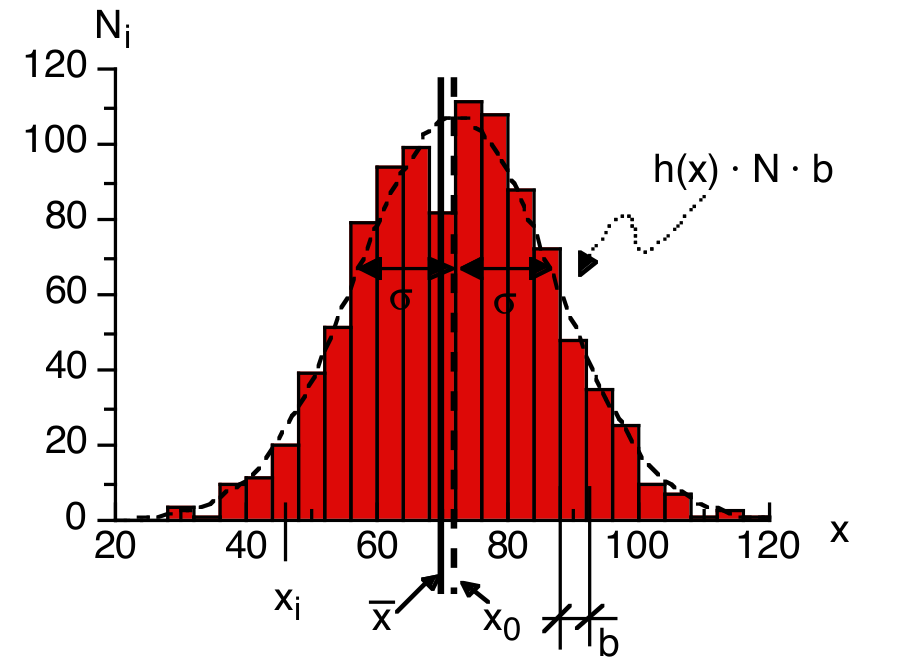
\includegraphics[width=0.5\textwidth]{images/gauss.png}
    \caption{Histogramm mit Gauss'scher Normalverteilung. \textbf{Quelle}: Skript ``Arbeitsunterlagen'', p13.}
    \label{fig:gauss}
\end{figure}

Die in Abbildung \ref{fig:gauss} gezeigte Kurve $h(x)$ kann beschrieben werden mit:
\begin{gather}
    h(x) = \frac{1}{\sqrt{2\pi\sigma^2}} \cdot exp\left(- \frac{(x-x_0)^2}{2\sigma^2}\right) \\
    \text{wobei} \\
    x_0 \text{ Erwartungswert (wahrer Wert)} \\
    \sigma \text{ Standardabweichung}
\end{gather}

F\"ur steigendes N geht der gemessene Mittelwert $\overline{x}$ gegen den wahren Wert $x_0$.

\begin{equation}
    \text{experimentelle Standardabweichung: } s = \sqrt{\frac{\sum_1^N{(x_i-\overline{x})^2}}{N-1}}
\end{equation}

Die  experimentelle Standardabweichung  $s$ konvergiert  f\"ur $N  \rightarrow
D\infty $ gegen $\sigma$. er Fehler der Einzelmessung $s_{T_i}$ und der Fehler
$s_{\overline{T}}$ des Mittelwertes stehen in folgender Beziehung:

\begin{equation}
    s_{\overline{T}} = \frac{s_{T_i}}{\sqrt{N}}
\end{equation}

Daraus  folgt z.B.,  dass der  Mittelwert einer  Serie von  100 Messungen  die
zehnfache Genauigkeit der Einzelmessung aufweist.


\subsubsection{Regression (``Fitten'')}

\begin{gather}
    \chi^2(a_0,a_1,...) = \sum_{1}^{N}{\frac{[y_i - f(x_i,a_0,a_1,...)]^2}{\sigma_i^2}} \text{: minimal}\\
    \text{wobei:} \\
    f(x,a_0,a_1) \text{: gegebene Gesetzm\"assigkeit/Funktion} \\
    x_i,y_i \text{: Messwertpaare}
\end{gather}

\begin{itemize}
    \item
        \emph{Nichtlineare   Funktionen  $f$}: Nichtlineare   Regression. Gute
        Startwerde erforderlich f\"ur $a_i$.
    \item
        \emph{Polynomiale Funktion  $f$}: Lineare Regression. Unabh\"angig vom
        Startwert  existiert  lediglich  ein Minimum. Startwerte  f\"ur  $a_i$
        daher nicht relevant.
    \item
        \emph{Verwendung  einer  Software  zum  Fitten}:  x-Werte  sollen  als
        Stellgr\"osse   (absolute  genau)   betrachtet  werden,   y-Werte  als
        fehlerbehaftet (Messgr\"osse).
\end{itemize}

Berechnung des Fehlers $\sigma_i$ der Einzelmessung aus dem Fit:

\begin{equation}
    \sigma_i = \sqrt{\frac{\sum_1^N{(y_i-f(x_i,a_0,a_1,...)})^2}{N - m}}
\end{equation}

Wobei $N$  die Anzahl  Messergebnisse, $m$  die Anzahl  Parameter $a_0,...a_m$
bezeichnet. Die Parameter $a_i$ m\"ussen aus dem Fit herausgelesen werden.


% **************************************************************************** %
\subsection{Fehlerfortpflanzung und Auswertung}
% **************************************************************************** %

\subsubsection{Indirekte Messung, das Fehlerfortpflanzungsgesetz}

Seien:
\begin{gather}
    \text{Resultatgr\"osse: } R = R(x,y,z,...) \\
    \text{Argumente (gemessen und/oder aus Literatur): } \\
    x = \overline{x} \pm s_{\overline{x}} \\
    y = \overline{y} \pm s_{\overline{y}} \\
    z = \overline{z} \pm s_{\overline{z}}
\end{gather}

Gesucht: Mittelwert $\overline{R}$ und mittlerer Fehler $s_{\overline{R}}$

\begin{equation}
    \overline{R} = R(\overline{x},\overline{y},\overline{z},...)
\end{equation}

Mittlerer,  absoluter  Fehler  (statistischer Fehler): Bestimmen  mittels  dem
\emph{Gauss'schen Fehlerfortpflanzungsgesetz}:

\begin{gather}
    s_{\overline{R}} = \sqrt{ \left( \frac{\partial R}{\partial x} \biggr\rvert_{\overline{R}} \cdot s_{\overline{x}}\right)^2
                            + \left( \frac{\partial R}{\partial y} \biggr\rvert_{\overline{R}} \cdot s_{\overline{y}}\right)^2
                            + \left( \frac{\partial R}{\partial z} \biggr\rvert_{\overline{R}} \cdot s_{\overline{z}}\right)^2
                            + ... }
\end{gather}

Wobei  $\frac{\partial R}{\partial  z}  \bigr\rvert_{\overline{R}}$ f\"ur  die
partielle Ableitung  der Funktion $R$  nach der Variablen $x$,  ausgewertet an
der Stelle  der Mittelwerte  $\overline{x}, \overline{y}, \overline{z},  ... $
steht.

Der Fehler $\pm s_R$ bezeichnet die Intervallbreite, in welcher der wahre Wert
mit 68 \% Wahrscheinlichkeit liegt.

\subsubsection{Spezialf\"alle des Fehlerfortpflanzungsgesetzes (``Rezepte'')}

\begin{itemize}
    \item
        \emph{Addition  und Subtraktion}:  $s_R  =  \sqrt{s_x^2 +  s_y^2}$. Es
        werden die absoluten Fehler quadratisch addiert.
    \item
        \emph{Multiplikation   und   Division}:   $r_R   =   \frac{s_R}{R}   =
        \sqrt{(\frac{s_x}{x})^2   +   (\frac{s_y}{y})^2}   =   \sqrt{r_x^2   +
        r_y^2}$. Es werden die relativen Fehler quadratisch addiert.
    \item
        \emph{Potenzen}: $r_R = \frac{s_R}{R} =  n * r_x$. Der relative Fehler
        der Messgr\"osse wird mit dem Exponenten multipliziert.
\end{itemize}

In Endresultaten sind immer absolute Fehler anzugeben.
